\documentclass[border=5pt]{standalone}
\usepackage{tikz}
\usepackage{amsmath}
\begin{document}
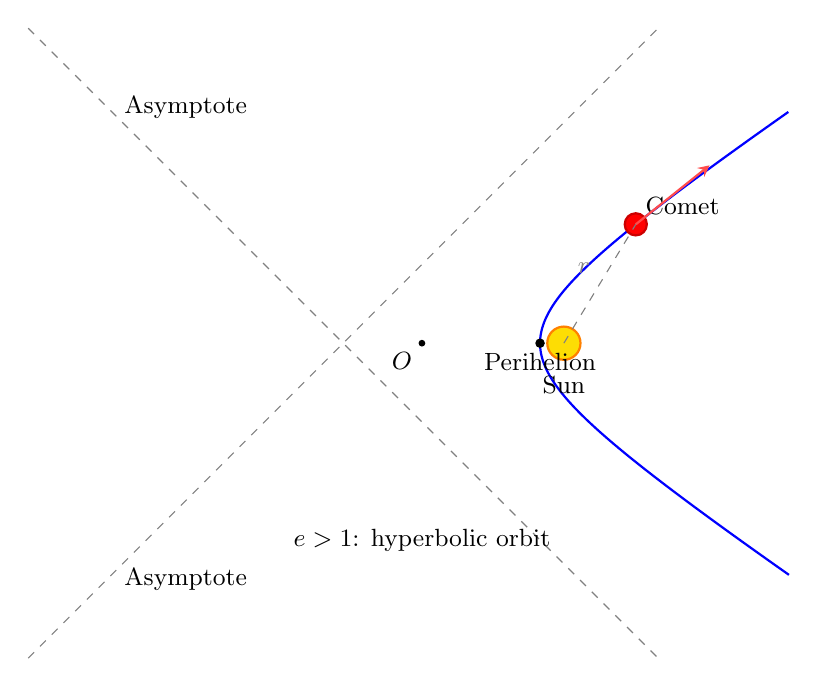
\begin{tikzpicture}[scale=1.0, >=stealth]
  % Hyperbolic comet trajectory: one branch of hyperbola
  % Sun at focus, comet approaching and leaving

  % Asymptotes (approach/departure directions)
  \draw[dashed, gray, thin] (-5, -4) -- (3, 4);
  \draw[dashed, gray, thin] (-5, 4) -- (3, -4);

  % Hyperbola branch (right side, comet path)
  \draw[blue, thick, domain=-1.8:1.8, samples=200]
    plot ({1.5*cosh(\x)}, {sinh(\x)});

  % Sun at focus
  \pgfmathsetmacro{\c}{sqrt(1.5*1.5 + 1)}
  \filldraw[yellow!80!orange, draw=orange, thick] (\c, 0) circle (6pt);
  \node[below, font=\small] at (\c, -0.3) {Sun};

  % Comet on trajectory
  \pgfmathsetmacro{\tx}{1.2}
  \pgfmathsetmacro{\cx}{1.5*cosh(\tx)}
  \pgfmathsetmacro{\cy}{sinh(\tx)}
  \filldraw[red, draw=red!80!black, thick] (\cx, \cy) circle (4pt);
  \node[above right, font=\small] at (\cx, \cy) {Comet};

  % Velocity vector (tangent to curve)
  \pgfmathsetmacro{\vx}{1.5*sinh(\tx)}
  \pgfmathsetmacro{\vy}{cosh(\tx)}
  \pgfmathsetmacro{\vlen}{sqrt(\vx*\vx + \vy*\vy)}
  \draw[->, thick, red!70] (\cx, \cy) -- ++({1.2*\vx/\vlen}, {1.2*\vy/\vlen});

  % Distance to focus
  \draw[dashed, gray, thin] (\c, 0) -- (\cx, \cy);
  \node[above left, font=\small, gray] at ({(\c+\cx)/2}, \cy/2) {$r$};

  % Perihelion
  \filldraw[black] (1.5, 0) circle (1.5pt) node[below, font=\small] {Perihelion};

  % Vertex
  \filldraw[black] (0,0) circle (1pt) node[below left, font=\small] {$O$};

  % Labels
  \node[font=\small] at (-3, 3) {Asymptote};
  \node[font=\small] at (-3, -3) {Asymptote};

  % Eccentricity label
  \node[font=\small] at (0, -2.5) {$e > 1$: hyperbolic orbit};
\end{tikzpicture}
\end{document}
